\documentclass[conference,onecolumn]{IEEEtran}
\usepackage{cite}
\usepackage{amsmath,amssymb,amsfonts}
\usepackage{graphicx}
\usepackage{textcomp}
\usepackage{xcolor}
\usepackage{booktabs,array}
\usepackage{newtxtext,newtxmath}
\usepackage{url}
\usepackage[hidelinks]{hyperref}
\usepackage{tikz}
\usetikzlibrary{arrows.meta,positioning,fit}
\graphicspath{{figures/}}
\newcommand{\KiB}{\,\mathrm{KiB}}
\newcommand{\MiB}{\,\mathrm{MiB}}
\newcommand{\codeurl}{https://github.com/mahaswint/cs5290/tree/main/pim-reproduction}
\title{Baseline Results: PIM-malloc Reproduction and Maintained Controls}
\author{\IEEEauthorblockN{CS5290 Project Group}}\begin{document}\maketitle
\section{Original artifact baseline}
These results reproduce the paper's allocation microbenchmark using the preserved released runtime, not the repaired contribution runtime. The reported paper-compatible aggregation is batch completion time divided by 128 requests/tasklet. Maximum absolute deviation from a printed label is 7.20\%. The original WRAM layout permits 256 KiB and therefore does not demonstrate physical 64 KiB fit.
\begin{table}[!htbp]
\caption{Original Figure 15 artifact reproduction: batch time divided by 128 requests per tasklet, in microseconds.}\label{tab:baseline}
\centering\small
\begin{tabular}{rrrrrrr}\toprule
Tasklets & Bytes & Paper buddy & Measured buddy & Paper SW & Measured SW & Buddy/SW \\ \midrule
1 & 32 & 630 & 584.66 & 6.9 & 6.99 & 83.66 \\
1 & 256 & 520 & 492.92 & 32 & 32.12 & 15.35 \\
1 & 4096 & 350 & 362.71 & 310 & 312.71 & 1.16 \\
16 & 32 & 13000 & 13026.39 & 51 & 51.86 & 251.17 \\
16 & 256 & 11000 & 10911.77 & 430 & 457.72 & 23.84 \\
16 & 4096 & 7700 & 7810.92 & 6700 & 6808.97 & 1.15 \\
\bottomrule\end{tabular}
\par\vspace{2pt}{\footnotesize The original simulator layout is preserved here. These latencies are separate from the repaired allocator and 64 KiB WRAM configuration used for contributions.}
\end{table}

\begin{figure}[!htbp]
\centering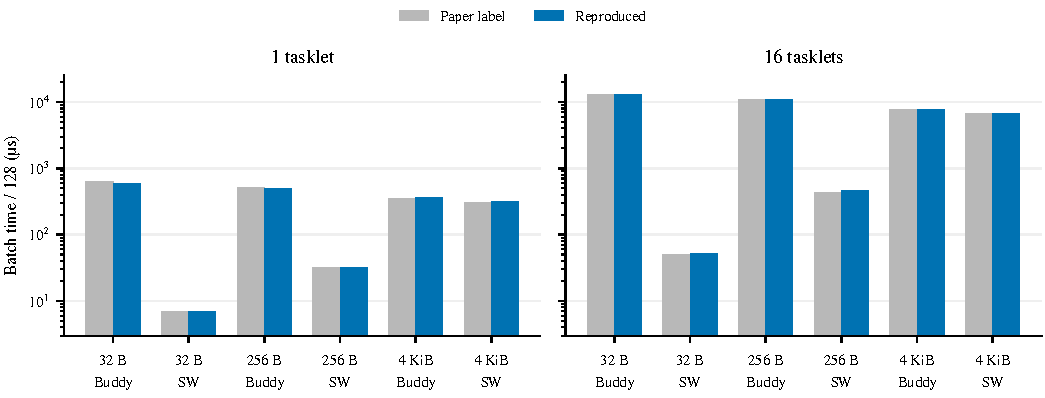
\includegraphics[width=\textwidth]{baseline-reproduction.pdf}
\caption{Original paper labels and reproduced allocator latencies.}\label{fig:base-extract}
\end{figure}

\section{Maintained baseline used for contributions}
Free/bitmap routing and empty-page reclamation are repaired identically in all maintained variants. The contribution runtime caps WRAM addresses at 65,536 B. The final baseline is scan fixed-2, which limits only completely empty retained pages/class. It uses a 32 MiB payload heap and 256 KiB empty-byte budget/tasklet. Its raw times are the B columns below; the adjacent contribution columns provide context. These values must not be merged with the original artifact as though only one optimization changed.
\begin{table}[!htbp]
\caption{Final work runtime (milliseconds) for every stage on five complementary cases.}\label{tab:final-main}
\centering\small
\begin{tabular}{lrrrrrrr}\toprule
Case & B & IA & IF & SA & SF & PA & PF \\ \midrule
Larson 8--4095 B (4T) & 160.089 & 164.537 & 159.826 & 24.026 & 19.894 & 19.172 & 16.255 \\
CloudPhysics cache (4T) & 122.773 & 122.925 & 122.784 & 114.586 & 114.528 & 113.023 & 113.075 \\
Larson 8--8191 B (4T) & 320.457 & 342.572 & 331.666 & 216.369 & 232.613 & 204.807 & 188.202 \\
Gowalla churn (4T) & 148.847 & 26.172 & 24.961 & 26.918 & 25.830 & 26.954 & 25.827 \\
PrIM selection (4T) & 14.134 & 14.180 & 14.180 & 14.135 & 14.135 & 14.133 & 14.133 \\
\bottomrule\end{tabular}
\par\vspace{2pt}{\footnotesize B: scan fixed-2; I: indexed; S: indexed plus 64 KiB slabs; P: indexed plus slabs plus pinned metadata. A uses adaptive interval 64; F retains at most two empty spans/class. All rows use four tasklets.}
\end{table}

\begin{table}[!htbp]
\caption{Final paper-derived cases: the baseline and both full-stack policies.}\label{tab:paper-final}
\centering\small
\begin{tabular}{lrrrrrr}\toprule
Case & B work (ms) & PA work (ms) & PF work (ms) & PA speedup & PF speedup & PF total speedup \\ \midrule
Gowalla linked blocks (4T) & 19.330 & 15.479 & 15.198 & 1.249 & 1.272 & 1.335 \\
Gowalla growing arrays (4T) & 5.752 & 5.845 & 5.494 & 0.984 & 1.047 & 1.070 \\
KV growth replay (4T) & 24.382 & 19.657 & 19.625 & 1.240 & 1.242 & 1.210 \\
32 B microbenchmark (1T) & 0.875 & 1.077 & 0.990 & 0.813 & 0.884 & 0.799 \\
32 B microbenchmark (16T) & 6.938 & 5.719 & 5.648 & 1.213 & 1.228 & 1.105 \\
256 B microbenchmark (1T) & 2.076 & 2.005 & 1.925 & 1.035 & 1.079 & 0.994 \\
256 B microbenchmark (16T) & 34.201 & 27.750 & 27.641 & 1.232 & 1.237 & 1.192 \\
4 KiB microbenchmark (1T) & 20.912 & 1.858 & 1.778 & 11.255 & 11.763 & 1.512 \\
4 KiB microbenchmark (16T) & 508.474 & 22.335 & 22.243 & 22.766 & 22.860 & 6.746 \\
\bottomrule\end{tabular}
\par\vspace{2pt}{\footnotesize Graph cases are reduced ports; KV is an allocation-only replay and excludes attention/serving. Original request sizes and 128 microbenchmark requests/tasklet are retained. Values below one are regressions.}
\end{table}

\section{Available data}
The accompanying tables include the original six paper/measured pairs, the final baseline conditions and exact phase/traffic definitions. All contribution speedups use the matching stage control. Simulated frequency is 350 MHz. Graphs are reduced ports and KV is allocation-only.\end{document}
